\documentclass[a4paper,12pt,obeyspaces,spaces,hyphens]{article}

\usepackage{agenda}
\usepackage{colortbl}
\usepackage{xcolor}
\usepackage{calc}

\hypersetup{pdftitle={Embedded Linux system development training},
  pdfauthor={Free Electrons}}

\renewcommand{\arraystretch}{2.0}

\begin{document}

\thispagestyle{fancy}

\setlength{\arrayrulewidth}{0.8pt}

\begin{center}
\LARGE
Embedded Linux system development training\\
\large
5-day session
\end{center}
\vspace{1cm}

\small
\newcolumntype{g}{>{\columncolor{fedarkblue}}m{4cm}}
\newcolumntype{h}{>{\columncolor{felightblue}}X}

\arrayrulecolor{lightgray} {
  \setlist[1]{itemsep=-5pt}
  \begin{tabularx}{\textwidth}{|g|h|}
    {\bf Title} & {\bf Embedded Linux system development training} \\
    \hline

    {\bf Overview} &
	Bootloaders \par
    Kernel (cross) compiling and booting \par
	Block and flash filesystems \par
    C library and cross-compiling toolchains \par
	Lightweight building blocks for embedded systems \par
    Embedded system development tools \par
	Embedded application development and debugging \par
	Implementing real-time requirements in embedded Linux systems \par
	Practical labs with the ARM based SAMA5D3 Xplained board from Atmel \\
    \hline
    {\bf Materials} &
    Check that the course contents correspond to your needs:
    \newline \url{http://free-electrons.com/doc/training/embedded-linux}. \\
    \hline

    {\bf Duration} & {\bf Five} days - 40 hours (8 hours per day).
    \newline 50\% of lectures, 50\% of practical labs. \\
    \hline

    {\bf Trainer} & One of the engineers listed on:
    \newline \url{http://free-electrons.com/training/trainers/}\\
    \hline

    {\bf Language} & Oral lectures: English, French, German or Polish.
    \newline Materials: English.\\
    \hline

    {\bf Audience} & People developing devices using the Linux kernel
    \newline People supporting embedded Linux system developers. \\
    \hline

    {\bf Prerequisites} &
    {\bf Knowledge and practice of UNIX or GNU/Linux commands}
    \newline People lacking experience on this topic should get
    trained by themselves, for example with our freely available
    on-line slides:
    \newline \url{http://free-electrons.com/docs/command-line/}. \\
    \hline
  \end{tabularx}

  \begin{tabularx}{\textwidth}{|g|h|}
    {\bf Required equipment} &
    {\bf For on-site sessions only}
    \newline Everything is supplied by Free Electrons in public sessions.
    \begin{itemize}
    \item Video projector
    \item PC computers with at least 2 GB of RAM, and Ubuntu Linux
    installed in a {\bf free partition of at least 20 GB. Using Linux
      in a virtual machine is not supported}, because of issues
    connecting to real hardware.
    \item We need Ubuntu Desktop 14.04 (32 or 64 bit, Xubuntu and
    Kubuntu variants are fine). We don't support other
    distributions, because we can't test all possible package versions.
    \item {\bf Connection to the Internet} (direct or through the
    company proxy).
    \item {\bf PC computers with valuable data must be backed up}
    before being used in our sessions.  Some people have already made
    mistakes during our sessions and damaged work data.
    \end{itemize}\\
    \hline

    {\bf Materials} & Print and electronic copies of presentations and
    labs.
    \newline Electronic copy of lab files.\\
    \hline

\end{tabularx}}
\normalsize

\feagendatwocolumn
{Hardware}
{
	Using the Atmel SAMA5D3 Xplained board in all practical labs
	SAMA5D36 (Cortex A5) CPU from Atmel, which features:

  \begin{itemize}
  \item USB powered
  \item 256 MB DDR2 RAM
  \item 256 MB NAND flash
  \item 2 Ethernet ports (Gigabit + 100 Mbit)
  \item 2 USB 2.0 host ports
  \item 1 USB device port
  \item 1 MMC/SD slot
  \item 3.3 V serial port (like Beaglebone Black)
  \item Arduino R3-compatible header
  \item Misc: JTAG, buttons, LEDs
  \end{itemize}
}
{}
{
  \begin{center}
    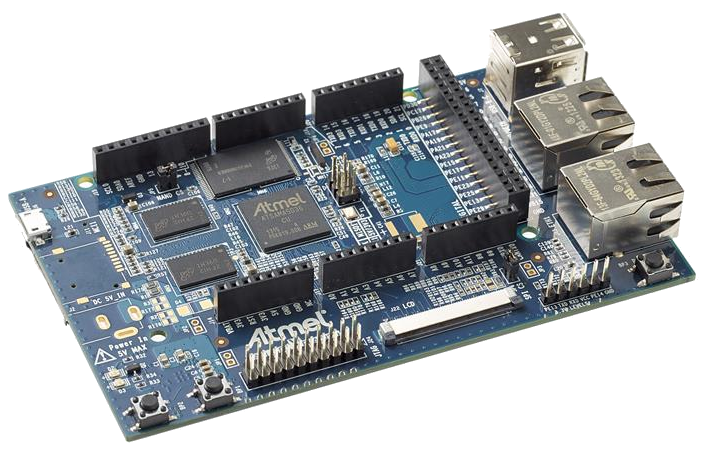
\includegraphics[height=5cm]{../slides/xplained-board/xplained-board.png}
  \end{center}
}

\section{Day 1 - Morning}

\feagendaonecolumn
{Lecture - Introduction to embedded Linux}
{
  \begin{itemize}
  \item Advantages of Linux versus traditional embedded operating systems.
        Reasons for choosing Linux.
  \item Global picture: understanding the general architecture of an
        embedded Linux system.Overview of the major components in a typical
        system.
  \end{itemize}
  {\em The rest of the course will study each of these components in detail.}
}
\\
\feagendatwocolumn
{Lecture - Embedded Linux development environment}
{
  \begin{itemize}
  \item Operating system and tools to use on the development
        workstation for embedded Linux development.
  \item Desktop Linux usage tips.
  \end{itemize}
}
{Lecture - Cross-compiling toolchain and C library}
{
  \begin{itemize}
  \item What's inside a cross-compiling toolchain
  \item Choosing the target C library
  \item What's inside the C library
  \item Ready to use cross-compiling toolchains
  \item Building a cross-compiling toolchain with automated tools.
  \end{itemize}
}

\section{Day 1 - Afternoon}
\feagendatwocolumn
{Lab - Cross compiling toolchain}
{
  \begin{itemize}
  \item Configuring Crosstool-NG
  \item Executing it to build a custom uClibc toolchain.
  \end{itemize}
}
{Lecture - Bootloaders}
{
  {\em Using the Atmel SAMA5D3 Xplained board}
  \begin{itemize}
  \item Available bootloaders
  \item Bootloader features
  \item Installing a bootloader
  \item Detailed study of U-Boot
  \end{itemize}
}
\\

\feagendatwocolumn
{Lab - Bootloader and U-boot}
{
  \begin{itemize}
  \item Set up serial communication with the board.
  \item Configure, compile and install the first-stage bootloader
        and U-Boot on the Xplained board.
  \item Become familiar with U-Boot environment and commands.
  \item Set up TFTP communication with the board. Use TFTP U-Boot commands.
  \end{itemize}
}
{Lecture - Linux kernel}
{
  \begin{itemize}
  \item Role and general architecture of the Linux kernel
  \item Features available in the Linux kernel,
        with a focus on features useful for embedded systems
  \item Kernel user interface
  \item Getting the sources
  \item Understanding Linux kernel versions.
  \item Using the patch command
  \end{itemize}
}
\\

\section{Day 2 - Morning}

\feagendatwocolumn
{Lab - Kernel sources}
{
  \begin{itemize}
  \item Downloading kernel sources
  \item Apply kernel patches
  \end{itemize}
}
{Lecture – Configuring and compiling a Linux kernel}
{
  {\em Using the Atmel Xplained board}
  \begin{itemize}
  \item Kernel configuration.
  \item Useful settings for embedded systems.
  \item Native compiling.
  \item Generated files.
  \item Using kernel modules
  \end{itemize}
}

\feagendatwocolumn
{Lecture - Kernel cross-compiling}
{
  \begin{itemize}
  \item Kernel cross-compiling setup.
  \item Using ready-made configuration files for specific architectures and boards.
  \item Cross-compiling Linux  \end{itemize}
}
{Lab - Kernel cross-compiling and booting}
{
  {\em Using the Atmel Xplained board}
  \begin{itemize}
  \item Configuring the Linux kernel and cross-compiling it for the ARM board.
  \item Downloading your kernel on the board through U-boot's tftp client.
  \item Booting your kernel from RAM.
  \item Copying the kernel to flash and booting it from this location.
  \item Storing boot parameters in flash and automating kernel booting from flash.
  \end{itemize}
}

\section{Day 2 - Afternoon}

\feagendatwocolumn
{Lecture – Root filesystem in Linux}
{
  \begin{itemize}
  \item Filesystems in Linux.
  \item Role and organization of the root filesystem.
  \item Location of the root filesystem: on storage, in memory,
        from the network.
  \item Device files, virtual filesystems.
  \item Contents of a typical root filesystem.
  \end{itemize}
}
{Lecture - BusyBox}
{
  {\em Using the Atmel Xplained board}
  \begin{itemize}
  \item Detailed overview. Detailed features.
  \item Configuration, compiling and deploying.
  \end{itemize}
}

\feagendaonecolumn
{Lab – Tiny root filesystem built from scratch with BusyBox}
{
  {\em Using the Atmel Xplained board}
  \begin{itemize}
  \item Now build a basic root filesystem from scratch for your ARM system
  \item Setting up a kernel to boot your system on a workstation
        directory exported by NFS
  \item Passing kernel command line parameters to boot on NFS
  \item Creating the full root filesystem from scratch.
        Populating it with BusyBox based utilities.
  \item Creating device files and booting the virtual system.
  \item System startup using BusyBox /sbin/init
  \item Using the BusyBox http server.
  \item Controlling the target from a web browser on the PC host.
  \item Setting up shared libraries on the target and compiling
        a sample executable.
  \end{itemize}
}

\section{Day 3 - Morning}

\feagendaonecolumn
{Lab – Tiny root filesystem built from scratch with BusyBox}
{
   Continued from the previous afternoon.
}

\feagendatwocolumn
{Lecture - Block filesystems}
{
  \begin{itemize}
  \item Filesystems for block devices.
  \item Usefulness of journaled filesystems.
  \item Read-only block filesystems.
  \item RAM filesystems.
  \item How to create each of these filesystems.
  \item Suggestions for embedded systems.
  \end{itemize}
}
{Lab - Block filesystems}
{
  {\em Using the Xplained ARM board}
  \begin{itemize}
  \item Creating partitions on your block storage
  \item Booting a system with a mix of filesystems: SquashFS for
	applications, ext3 for configuration and user data, and
	tmpfs for temporary system files.
  \end{itemize}
}

\section{Day 3 - Afternoon}

\feagendatwocolumn
{Lecture - Flash filesystems}
{
  \begin{itemize}
  \item The Memory Technology Devices (MTD) filesystem.
  \item Filesystems for MTD storage: JFFS2, Yaffs2, UBIFS.
  \item Kernel configuration options
  \item MTD storage partitions.
  \item Focus on today's best solution, UBI and UBIFS:
	preparing, flashing and using UBI images.
  \end{itemize}
}
{Lab – Flash filesystems}
{
  {\em Using the SAMAD3 Xplained ARM board}
  \begin{itemize}
  \item Defining partitions in U-Boot for your internal
        flash storage instead of using raw offsets.
  \item Sharing these definitions with Linux.
  \item Creating a UBI image on your workstation, flashing
        it from U-Boot and booting your system on one of
        the UBI volumes with UBIFS. 
  \end{itemize}
}

\feagendaonecolumn
{Lecture – Leveraging existing open-source components in your system}
{
  \begin{itemize}
  \item Reasons for leveraging existing components.
  \item Find existing free and open source software components.
  \item Choosing the components.
  \item The different free software licenses and their requirements.
  \item Overview of well-known typical components used in
        embedded systems : graphical libraries and systems
        (framebuffer, Gtk, Qt, etc.), system utilities,
        network libraries and utilities, multimedia libraries, etc.
  \item System building: integration of the components.
  \end{itemize}
}

\section{Day 4 - Morning}

\feagendatwocolumn
{Lecture – Cross-compiling applications and libraries}
{
  \begin{itemize}
  \item Configuring, cross-compiling and installing applications and libraries.
  \item Details about the build system used in most open-source components.
  \item Overview of the common issues found when using these components.
  \end{itemize}
}
{Lab – Cross-compiling applications and libraries}
{
  {\em If enough time left}
  \begin{itemize}
  \item Building a system with audio libraries and a sound player application.
  \item Manual compilation and installation of several free software packages.
  \item Learning about common techniques and issues.
  \end{itemize}
}

\section{Day 4 - Afternoon}

\feagendatwocolumn
{Lecture - Embedded system building tools}
{
  \begin{itemize}
  \item Review of existing system building tools.
  \item Buildroot example.
  \end{itemize}
}
{Lab - System build with Buildroot}
{
  {\em Using the Atmel Xplained board}
  \begin{itemize}
  \item Using Buildroot to rebuild the same system as in the previous lab.
  \item Seeing how easier it gets.
  \item Optional: add a package to Buildroot.
  \end{itemize}
}

\section{Day 5 - Morning}

\feagendaonecolumn
{Lecture - Application development and debugging}
{
  \begin{itemize}
  \item Programming languages and libraries available.
  \item Overview of the C library features for application development.
  \item Build system for your application,
        how to use existing libraries in your application.
  \item Source browsers and Integrated Development Environments (IDEs).
  \item Debuggers. Debugging remote applications with gdb and gdbserver.
        Post-mortem debugging with core files.
  \item Code checkers, memory checkers, profilers.
  \end{itemize}
}

\feagendaonecolumn
{Lab – Application development and debugging}
{
  {\em On the Atmel Xplained board}
  \begin{itemize}
  \item Develop and compile an application relying on the ncurses library
  \item Using strace, ltrace and gdbserver to debug a crappy application
        on the remote system.
  \item Do post-mortem analysis of a crashed application.
  \end{itemize}
}


\section{Day 5 - Afternoon}

\feagendaonecolumn
{Lecture - Linux and real-time}
{
  {\em Very useful for many kinds of devices, industrial or multimedia systems.}
  \begin{itemize}
  \item Understanding the sources of latency in standard Linux.
  \item Soft real-time solutions for Linux: improvements included
        in the mainline Linux version.
  \item Understanding and using the latest RT preempt patches for
        mainline Linux.
  \item Real-time kernel debugging. Measuring and analyzing latency.
  \item Xenomai, a hard real-time solution for Linux: features, concepts,
        implementation and examples.
  \end{itemize}
}

\feagendaonecolumn
{Lab - Linux latency tests}
{
  \begin{itemize}
  \item Tests performed on the Xplained ARM board.
  \item Latency tests on standard Linux, with preemption options.
  \item Latency tests using the \code{PREEMPT_RT} kernel patchset.
  \item Setting up Xenomai.
  \item Latency tests with Xenomai.
  \end{itemize}
}

\end{document}

